\section{First-Divergence Token Event Diagnostic}
\label{sec:alignment}

The trace-bound diagnostic is based on a simple property of autoregressive
token sequences.  If two continuations differ as text, then after their longest
shared token prefix there is a first next-token choice at which they diverge.
We use that event as a diagnostic unit because it is the earliest tokenizer
native point at which a phrase, style, template, or semantic trajectory can
become distinguishable.

\begin{definition}[First-divergence event]
Let $u=(u_1,\ldots,u_m)$ and $v=(v_1,\ldots,v_n)$ be two token continuations
after a shared prompt prefix.  If $u\neq v$, their first-divergence position is
the smallest index $t$ for which $u_t\neq v_t$, treating end-of-sequence as a
token when one sequence is a strict prefix of the other.  The first-divergence
event is the next-token branch observed at that position.
\end{definition}

\begin{lemma}[First divergence of text differences]
\label{lem:first-divergence}
For any two distinct tokenized continuations produced by an autoregressive
tokenizer-based model, there exists a first-divergence position after their
longest shared token prefix.
\end{lemma}

\begin{proposition}[First-divergence reduction]
\label{prop:first-divergence-reduction}
Let a deterministic evidence rule partition tokenized continuations into two
or more observable classes.  If two continuations fall in different classes,
then the class distinction has at least one first-divergence event witness:
after the continuations' longest shared token prefix, their next-token branches
are different.
\end{proposition}

\begin{proposition}[Public-predicate spoofability under nonzero source density]
\label{prop:public-predicate-spoofability}
Let $A(x)\in\{0,1\}$ be a deterministic public predicate over final text, and
let $D$ be a source-mismatch proposal distribution.  If
$p=\Pr_{x\sim D}[A(x)=1]>0$, then rejection sampling from $D$ finds an
accepted source-mismatch example with expected $1/p$ predicate evaluations.
Such an accepted example is spoofing evidence against the predicate, not
protected success or codeword recovery.
\end{proposition}

Lemma~\ref{lem:first-divergence} is elementary, but it clarifies the role of
the diagnostic.  Proposition~\ref{prop:first-divergence-reduction} extends the
same observation from pairwise text differences to deterministic evidence
classes: any class distinction that appears in tokenized continuations must be
witnessed by some earliest branch.  If a provider-side trace records those
events and binds them to the final output, then the trace can expose
information that may be absent from a public final-text view.

\paragraph{Upper-bound role.}
The first-divergence diagnostic is an upper-bound measurement of model-side
controllability under event access.  If protected codewords cannot be recovered
from first-divergence traces, then a weaker public final-text-only substrate is
unlikely to recover the same keyed evidence.  If first-divergence traces do
recover codewords while public final text recovers none, the bottleneck is
public observability rather than the absence of event-level capacity.

\begin{figure}[t]
\centering
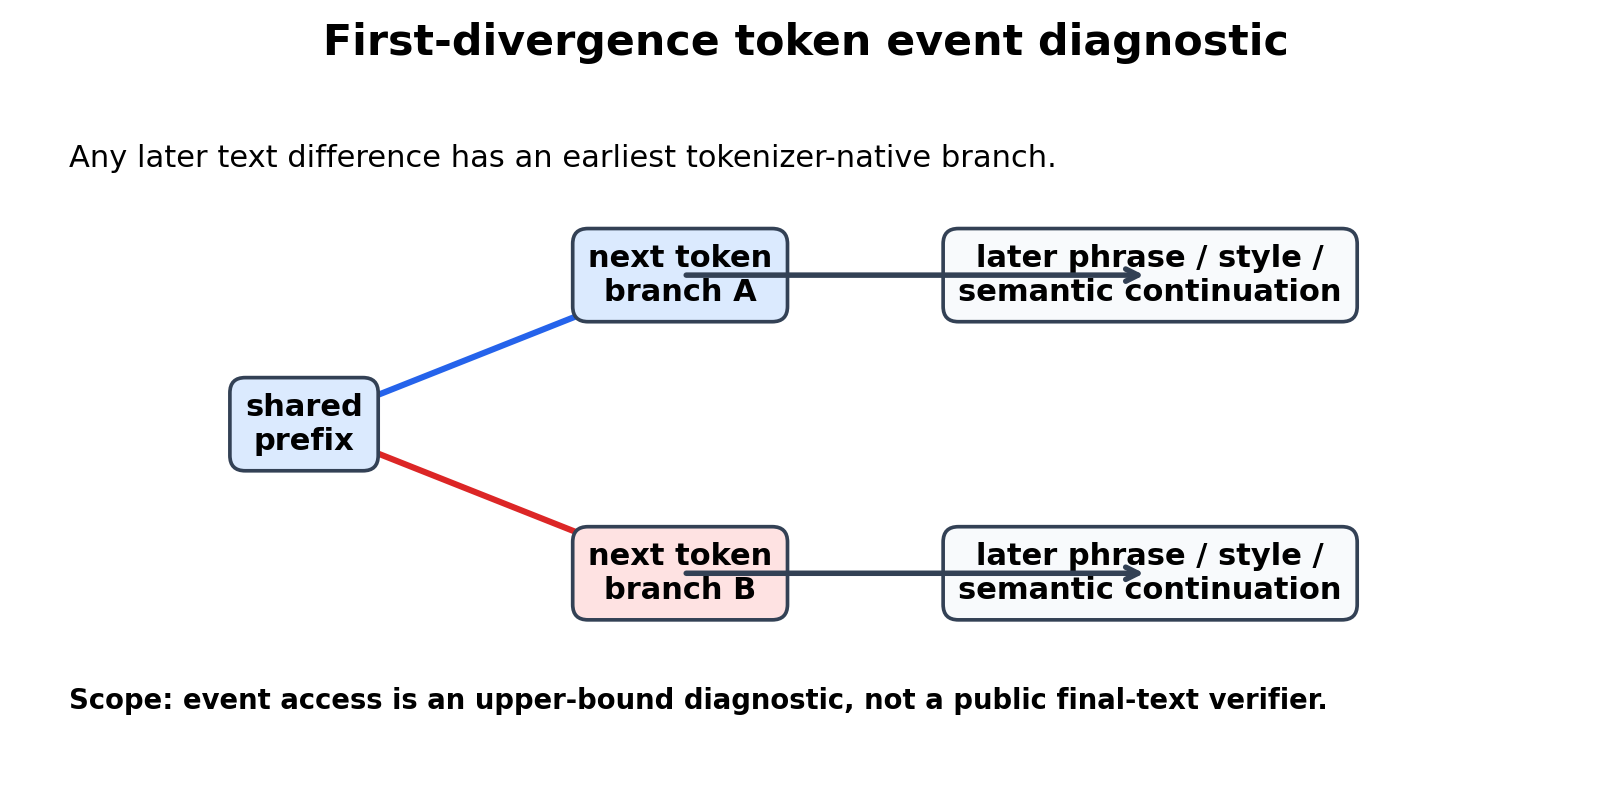
\includegraphics[width=\linewidth]{figures/figure_2_first_divergence_diagnostic.png}
\caption{First-divergence token events as a diagnostic unit.  The figure shows
how two continuations share a prefix before branching at a next-token event.
This is a trace-bound controllability diagnostic, not a public final-text
verifier and not public text-only verification success.}
\label{fig:first-divergence}
\end{figure}

\paragraph{Not a public verifier.}
The diagnostic is not a deployable public final-text verifier.  It assumes
provider-side event access and therefore belongs to the trace substrate in
Table~\ref{tab:substrate-taxonomy}.  It can support a cooperative trace-bundle
audit, but it does not by itself support copied-text verification,
rewritten-text verification, cryptographic provenance, or an ownership proof.

\paragraph{Why this matters for the experiments.}
The experiments below compare two views of the same broad phenomenon.  In the
trace-bound view, an authorized verifier observes selected first-divergence
token events and tests whether a protected codeword is recoverable under
controls.  In the public final-text view, a third party observes only text and
tries to recover or approximate the signal from shallow predicates.  The
verification substrate gap is the empirical separation between these views.

\paragraph{Why shallow predicates are not enough.}
Proposition~\ref{prop:public-predicate-spoofability} gives the minimal reason a
public final-text predicate with nonzero source-mismatch density is risky.  It
does not say that every public predicate is breakable, and it is not a
universal impossibility theorem.  It says that a predicate with an observable
accept region becomes a target for search.  In the current artifacts, the Qwen
raw P2 source-mismatch rate is 0.193455, the Qwen task-only rate is 0.195060,
and the Llama raw rate is 0.038798.  A direct rejection sampler would therefore
expect accepted source-mismatch examples after about 5.17, 5.13, and 25.8
predicate evaluations respectively, before any rewrite, surrogate ranking, or
guided optimization is applied.
